\newcommand{\docNome}{Manuale Utente}                          % NOME DEL DOCUMENTO
\newcommand{\docVersione}{1.1.0}                 % INSERIRE VERSIONE IN FORMATO x.y.z
\newcommand{\docStatus}{In lavorazione}          % AGGIORNARE SOLO QUANDO APPROVATO
\newcommand{\docUso}{Esterno}                           % INTERNO O ESTERNO
\newcommand{\docDestinatari}{
      Gruppo Sweven Team\\ %aggiungere altri con & Nome\\
      & Prof. Tullio Vardanega\\
      & Prof. Riccardo Cardin\\
      & Azienda Imola Informatica
} 
\newcommand{\docNomeTeam}{Sweven Team}
\newcommand{\docRedattori}{Irene Benettazzo \\
                            & Matteo Pillon}
\newcommand{\docVerificatori}{Samuele Rizzato \\
                              & Tommaso Berlaffa}
\newcommand{\docApprovazione}{Pan Qi Fan Andrea}
% Vesione dei documenti
\newcommand{\docVersionGlo}{\textit{v2.0.0}} % Glossario
\newcommand{\docVersionNdP}{\textit{v1.1.0}} % Norme di Progetto
\newcommand{\docVersionPdP}{\textit{v2.0.0}} % Piano di Progetto
\newcommand{\docVersionPdQ}{\textit{v2.0.0}} % Piano di Qualifica
\newcommand{\docVersionST}{\textit{v0.0.0}} % Specifica Tecnica
\newcommand{\docVersionAdR}{\textit{v2.0.0}} % Analisi dei Requisiti
\newcommand{\docVersionMU}{\textit{v0.0.0}} % Manuale Utente
\newcommand{\glossario}[1]{\textit{#1}\textsubscript{\textit{G}}}
\documentclass[12pt, a4paper,table]{article}
\usepackage[T1]{fontenc}
\usepackage[utf8]{inputenc}
\usepackage{lastpage}
\usepackage{hyperref}
\usepackage{fancyhdr}
\usepackage{fancyvrb}
\usepackage{geometry}
\usepackage{xcolor}
\usepackage{array}
\usepackage{graphicx}
\usepackage{float}
\usepackage{charter}
\usepackage{eurosym}
\usepackage{pdflscape}
\usepackage{longtable}
\hypersetup{
pdfborder = {0 0 0}
}
\geometry{a4paper,top=3cm,bottom=3cm,left=2cm,right=2cm}
\title{\textsc{\docNome}}
\author{}
\date{}
\definecolor{footer-gray}{HTML}{808080}
\pagestyle{fancy}
\fancyhf{}
\rhead{\textcolor{footer-gray}{\docNome} }
\lhead{\textcolor{footer-gray}{Sweven Team}}
\fancyfoot{}
\cfoot{\textcolor{footer-gray}{Pagina \thepage  \hspace{1pt} di \pageref*{LastPage}} }
\setcounter{tocdepth}{5}	%aggiunge paragrafi e sottoparagrafi all'indice
\setcounter{secnumdepth}{5}	%aggiunge numero indicizazzione a paragrafi e sottoparagrafi
\renewcommand*\contentsname{Indice}

\begin{document}
\maketitle
	\vspace{-3em}
	\begin{center}
	
\includegraphics[scale=0.50]{images/logo.jpg} \\
	\vspace{2em}
	\huge \textsc{\docNomeTeam}\\
	\normalsize \href{mailto:swe7.team@gmail.com}{swe7.team@gmail.com}\\
	\vspace{2em}
	\begin{tabular}{r|l}
		\multicolumn{2}{c}{ \textsc{Informazioni sul documento} } \\
		\hline
		\textbf{Versione}     & \docVersione\\
		\textbf{Uso}          & \docUso\\
        \textbf{Destinatari}  & \docDestinatari\\
		\textbf{Stato}        & \docStatus\\
		\textbf{Redattori}    & \docRedattori\\
		\textbf{Verificatori} & \docVerificatori\\
		\textbf{Approvatori} & \docApprovazione\\
	\end{tabular}
	\end{center}
    \vspace{3em}
    \begin{center}
        \LARGE{\textbf{Sintesi}} 
    \end{center}
    \normalsize{Guida per l'utente del prodotto \glossario{Chatbot}.}
	\thispagestyle{empty}   
	\newpage
\section*{Diario delle modifiche}
	\begin{center}
	\renewcommand{\arraystretch}{1.8} %aumento ampiezza righe
	\begin{longtable}{ |c|c|p{8em}|c|m{5em}|m{6em}| }
	\hline
	\textbf{Versione} & \textbf{Data} & \textbf{Descrizione} &  \textbf{Ruolo} &  \textbf{Autore} & \textbf{Verificatore}\\ %Aggiungere le nuove righe sopra la prima
	\hline % Se il nome non ci sta, metterlo a mano con aggiunta di \newline (esempio: Nome \newline Cognome)
    & 2022-08-09 & Scrittura \$3 & Amministratore & Irene \newline Benetazzo & \\ 
	\hline
	& 2022-08-08 & Scrittura \$1 & Amministratore & Irene \newline Benetazzo & \\ 
	\hline
	& 2022-07-21 & Creazione documento & Amministratore & Irene \newline Benetazzo & \\ 
	\hline
	\end{longtable}
	\end{center}
	\newpage
\tableofcontents
\newpage
\section{Introduzione}
\subsection{Scopo del documento}
Il Piano di Qualifica permette di raggruppare e ordinare le diverse modalità tramite le quali 
vengono effettuate le operazioni di verifica e di validazione necessarie per lo svolgimento corretto 
del progetto.

\subsection{Scopo del capitolato}
Lo scopo di tale progetto è quello di sviluppare un Chatbot che interfacciandosi con software aziendali spesso complessi e dispersivi, semplifichi i compiti che i dipendenti devono svolgere. In particolare vengono individuate le seguenti operazioni: 
\begin{itemize}
	\item Tracciamento della presenza in sede (\textbf{EMT}\textsubscript{G})
	\item Rendiconto attività svolte quotidianamente (\textbf{EMT}\textsubscript{G})
	\item Apertura del cancello aziendale (\textbf{MQTT}\textsubscript{G})
	\item Creazione di una riunione in un servizio esterno
	\item Servizio di ricerca documentale (\textbf{CMIS}\textsubscript{G})
	\item Creazione e tracciamento di bug (\textbf{Redmine}\textsubscript{G})
\end{itemize}

\subsection{Glossario}
Per assicurare la massima fruibilità e leggibilità del documento, il team SWEven ha deciso di creare un documento denominato \textit{Glossario} il cui scopo sarà quello di contenere le definizioni dei termini ambigui o specifici del progetto. Sarà possibile riconoscere i termini presenti al suo interno in quanto terminanti con la lettera \textit{G} posta come pedice della parola stessa. 
\subsection{Riferimenti}

\subsubsection{Normativi}
\begin{itemize}
	\item da scrivere
\end{itemize}

\subsubsection{Informativi}
\begin{itemize}
	\item \href{https://www.math.unipd.it/~tullio/IS-1/2021/Progetto/C1.pdf}{\color{blue} Capitolato di appalto C1 - BOT4ME}
\end{itemize}
\newpage
\section{Requisiti di Sistema}
\subsection{Requisiti Hardware minimi}
Per l'applicazione è necessario avere un computer che soddisfi le seguenti specifiche minime:
\begin{itemize}
    \item \textbf{Sistema Operativo:} Windows 10 (64bit), Ubuntu 20.04, MacOs 10.13 High Sierra
    \item \textbf{memoria (RAM):} 2GB
    \item \textbf{connessione internet:} attiva
\end{itemize}
\subsection{Requisiti minimi Web Application}
L'applicazione è accessibile tramite i browser:
\begin{itemize}
    \item \textbf{Google Chrome} a partire dalla versione 75
    \item \textbf{Microsoft Edge} a partire dalla versione 42
    \item \textbf{Mozilla Firefox} a partire dalla versione 69
    \item \textbf{Safari} a partire dalla versione 13
\end{itemize}

\newpage
\section{Inizio}
All'avvio dell'applicazione il chatbot, Bot4me, vi da il benvenuto con un messaggio suggerendo anche delle possibili funzionalità che è in grado di svolgere. 

\begin{figure}[H]
    \centering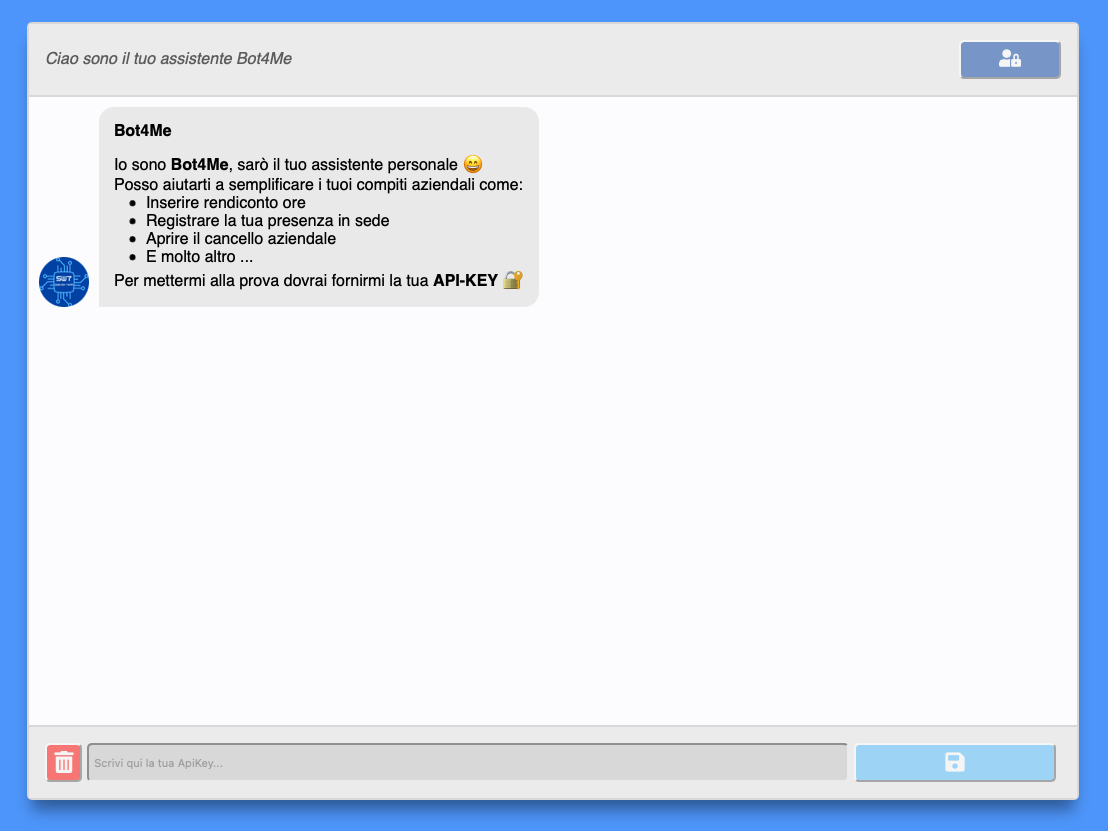
\includegraphics[width=0.9\textwidth, height=0.7\textheight, keepaspectratio]{images/schermata_avvio.png}
    \caption{Schermata Iniziale Bot4me}
\end{figure}

Inizialmente non si è loggati all'interno del sistema e per compiere qualsiasi tipo di operazione è necessario inserire un'\glossario{API-KEY} valida, ovvero che rispetti il formato suggerito da Imola Informatica, sarà poi compito del Server verificare se oltre che ad essere valida sia anche corretta per procedere con l'autenticazione. 

\subsection{Presentazione Grafica e Pulsanti}
\begin{itemize}
    \item Pulsante \textbf{Login / Logout:} in alto a destra il pulsante blu attualmente è solo per il login, dopo aver effettuato il login diventerà rosso per indicare il logout;
        \begin{figure}[H]
            \centering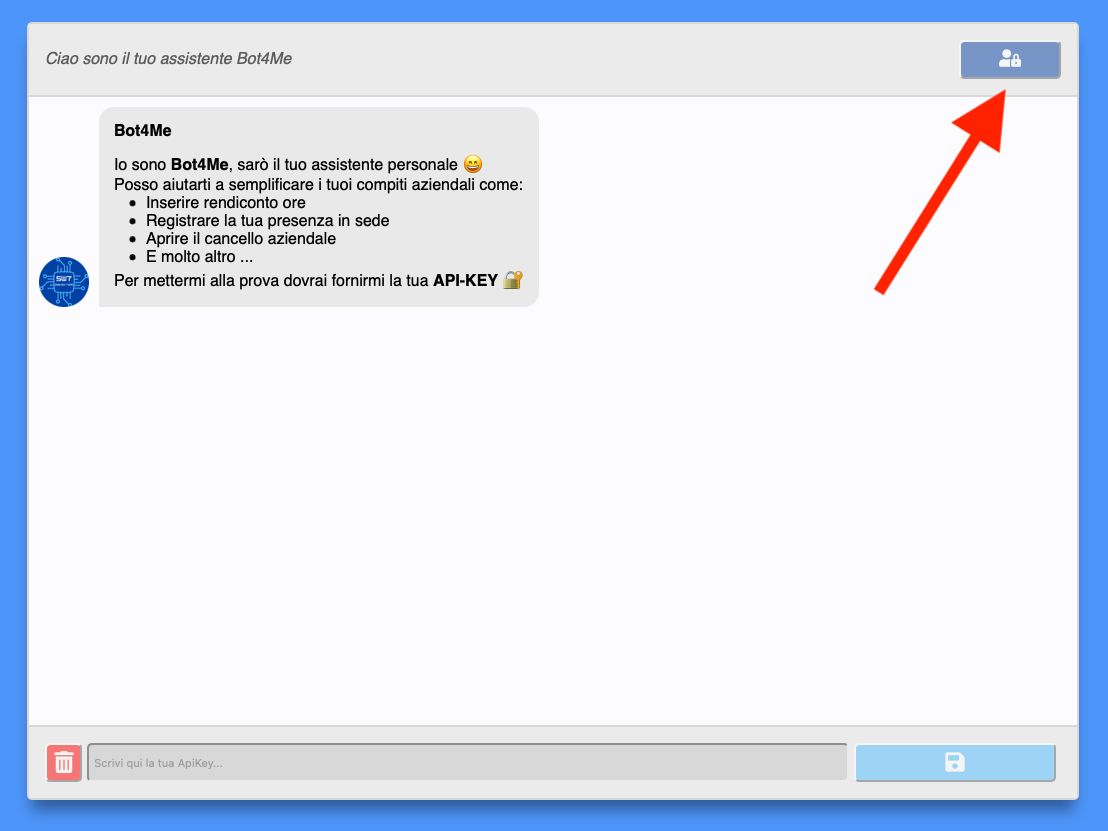
\includegraphics[width=0.8\textwidth, height=0.7\textheight, keepaspectratio]{images/schermata_pulsante_login.png}
            \caption{Pulsante - Login}
        \end{figure}
        \begin{figure}[H]
            \centering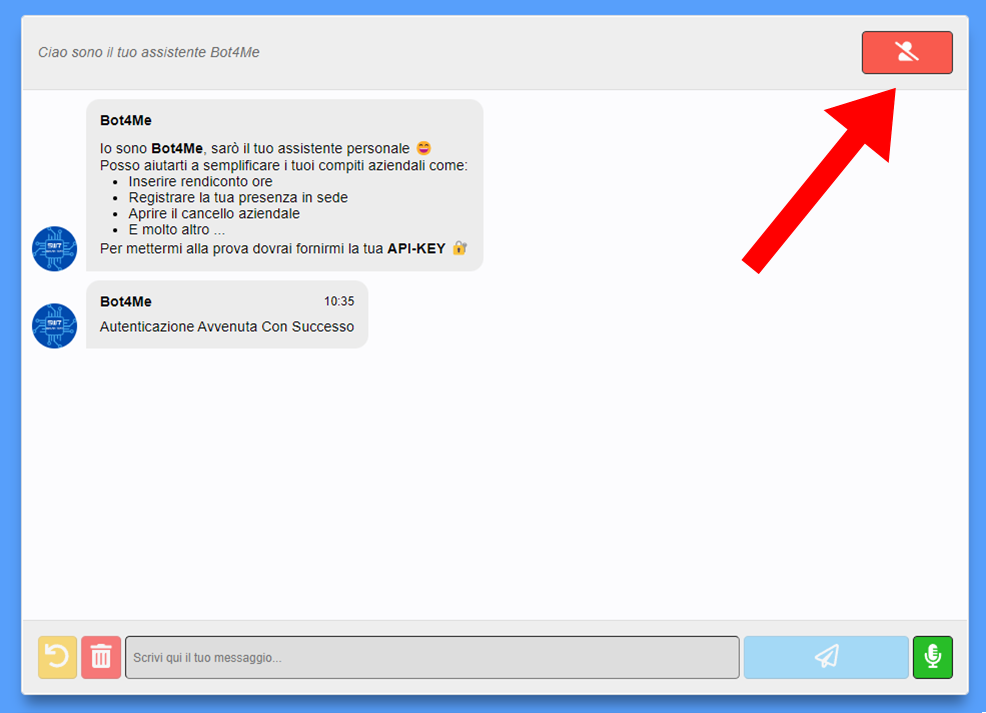
\includegraphics[width=0.8\textwidth, height=0.7\textheight, keepaspectratio]{images/schermata_pulsante_logout.png}
            \caption{Pulsante - Logout}
        \end{figure}
    \item Pulsante \textbf{Annulla:} in basso a sinistra il pulsante arancione serve per annullare la richiesta dell'operazione in corso, ritornando all'inizio. Non è possibile annullare un'operazione conclusa;
        \begin{figure}[H]
            \centering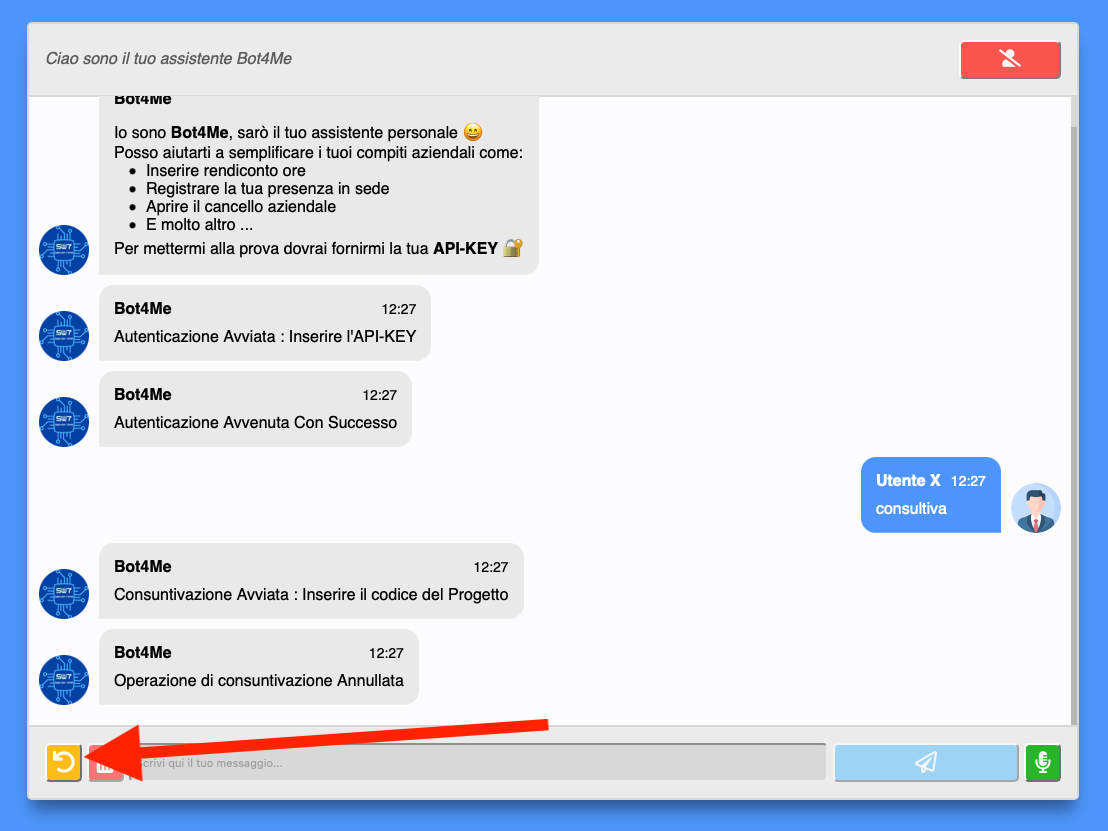
\includegraphics[width=0.8\textwidth, height=0.7\textheight, keepaspectratio]{images/schermata_pulsante_annulla.png}
            \caption{Pulsante - Annulla}
        \end{figure}
\newpage
    \item Pulsante \textbf{Elimina:} in basso a sinistra il pulsante rosso serve per cancellare ciò che si sta scrivendo, non è possibile premere il pulsante se la casella di testo è vuota;
        \begin{figure}[H]
            \centering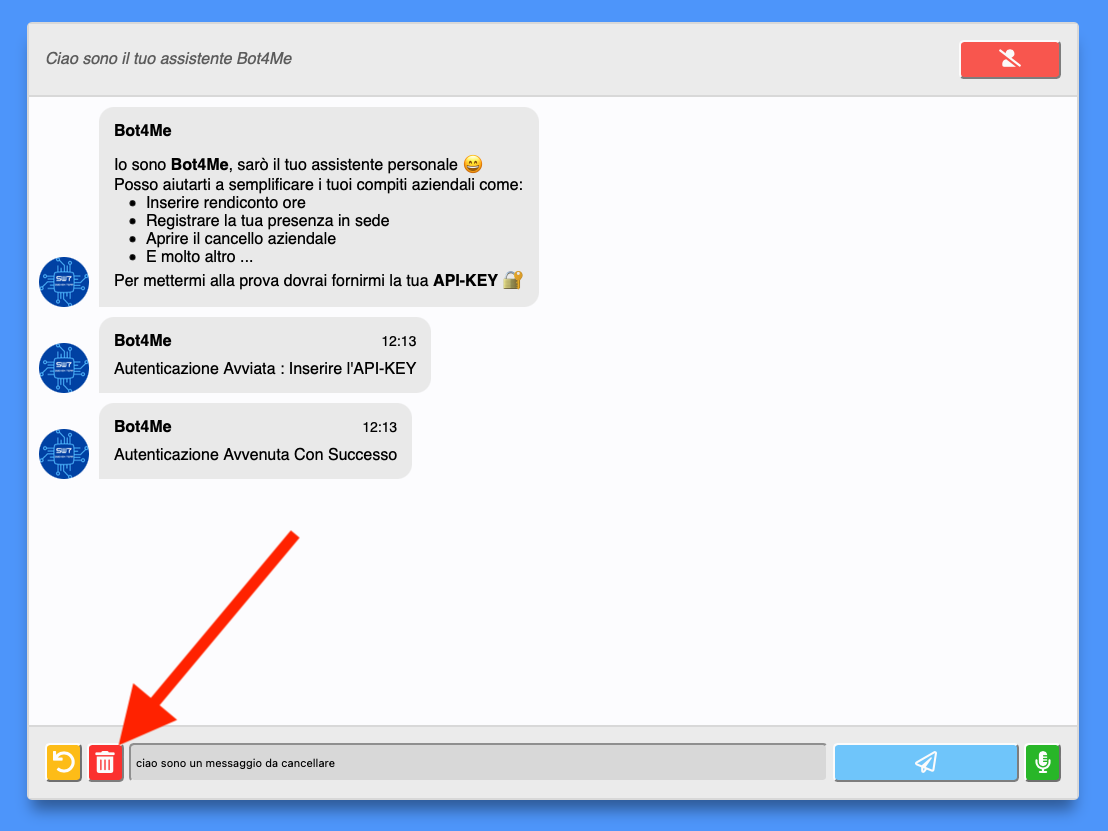
\includegraphics[width=0.8\textwidth, height=0.7\textheight, keepaspectratio]{images/schermata_pulsante_cancella.png}
            \caption{Pulsante - Elimina}
        \end{figure}
\newpage
    \item Pulsante \textbf{Invio:} in basso a destra il pulsante azzurro serve per inviare il messaggio scritto o alternativamente si può premere l'invio della tastiera;
        \begin{figure}[H]
            \centering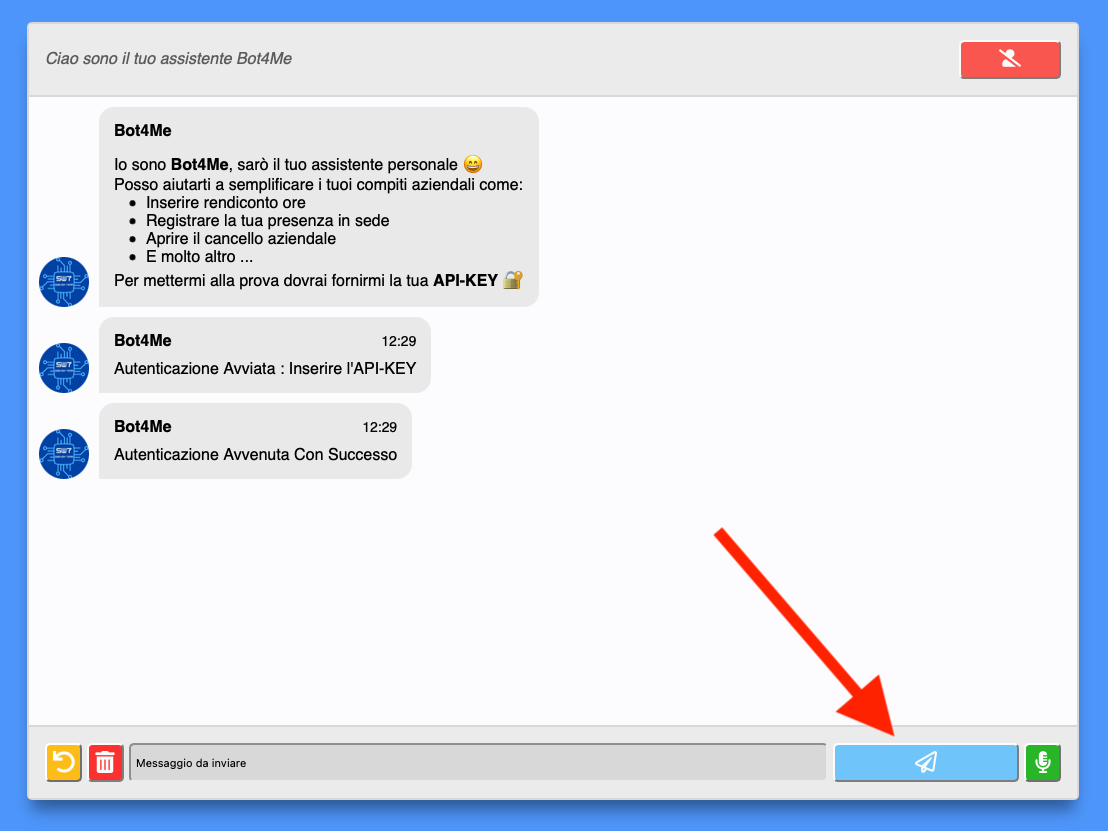
\includegraphics[width=0.8\textwidth, height=0.7\textheight, keepaspectratio]{images/schermata_pulsante_invio.png}
            \caption{Pulsante - Invio}
        \end{figure}
\newpage
    \item Pulsante \textbf{Vocale:} in basso a destra il pulsante verde serve per registrare vocalmente il messaggio che verrà automaticamente trascritto, con la possibilità di modificarlo manualmente nella casella di testo, e poi basterà cliccare sul pulsante azzurro o l'invio della tastiera; 
        \begin{figure}[H]
            \centering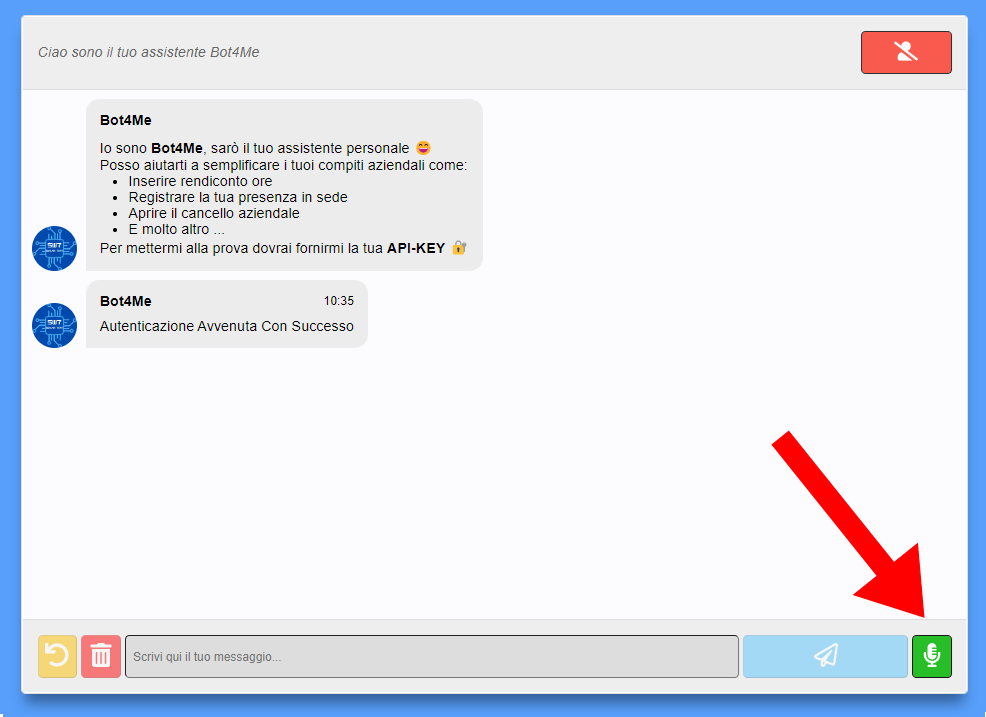
\includegraphics[width=0.8\textwidth, height=0.7\textheight, keepaspectratio]{images/schermata_pulsante_vocale.png}
            \caption{Pulsante - Vocale}
        \end{figure}

        \begin{figure}[H]
            \centering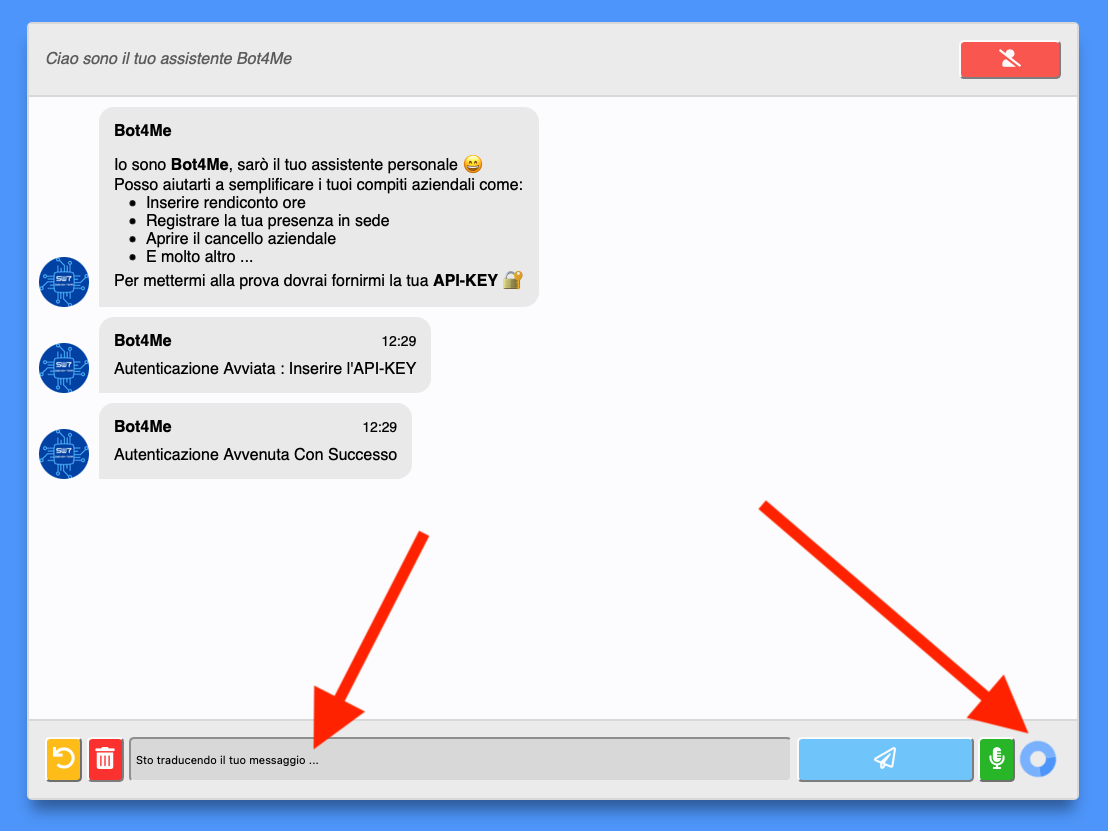
\includegraphics[width=0.8\textwidth, height=0.7\textheight, keepaspectratio]{images/schermata_pulsante_vocale_trascrizione.png}
            \caption{Trascrizione Messaggio Vocale}
        \end{figure}

\newpage
    \item Pulsante \textbf{Salva:} in basso a destra il pulsante azzurro con il simbolo di salvataggio, che prende il posto del pulsante d'invio e vocale, permette di salvare la propria \glossario{api-key} così da effettuare il processo di autenticazione.
    \begin{figure}[H]
        \centering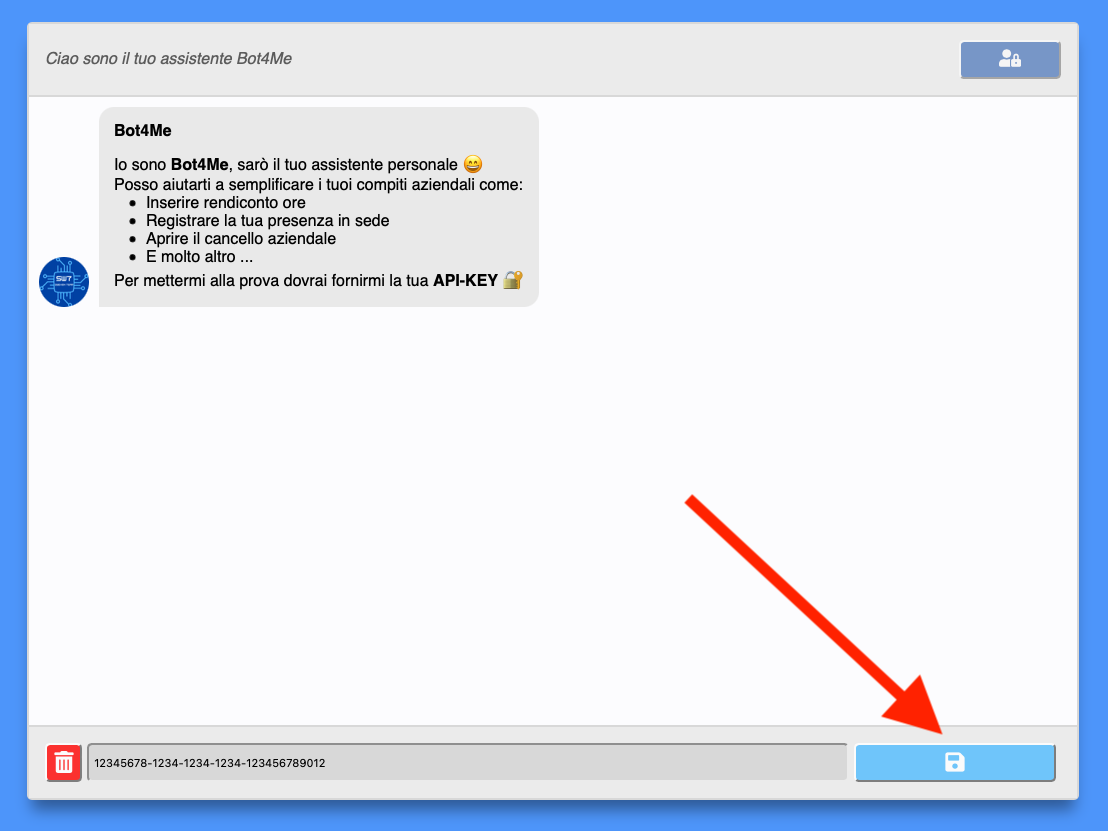
\includegraphics[width=0.8\textwidth, height=0.7\textheight, keepaspectratio]{images/schermata_pulsante_salva_API_KEY.png}
        \caption{Pulsante - Salva}
    \end{figure}
\end{itemize}

\newpage
\subsection{Autenticazione}
Per autenticarsi verrà chiesto di inserire la propria \glossario{API-KEY} di autenticazione dopo l'avvio dell'applicazione, se errata verrà comunicato che la richiesta è fallita, perchè l'\glossario{API-KEY} risulta essere errata. Il chatbot verrà dunque ricaricato e si potrà effettuare un nuovo tentativo; se risultasse essere corretta Bot4me comunica all'utente che l'autenticazione è avvenuta con successo e che può iniziare ad utilizzare i servizi che offre. 
Dopo l'autenticazione il pulsante in alto a destra diventerà di colore rosso con il simbolo di logout.
Se l'utente ricarica la pagina web, avviene un cambio di \glossario{UUID} e possono verificarsi due scenari: 
\begin{itemize}
    \item se l'utente ha effettuato il login in precedenza: la sua \glossario{API-KEY} risulta essere salvata all'interno del \glossario{Local-Storage} del browser, verrà dunque caricata all'interno della casella di testo e l'utilizzatore dell'applicazione potrà decidere se salvarla, tramite il bottone azzurro dotato dell'icona di salvataggio, effettuando così il login, oppure se modificarla e in seguito effettare l'autenticazione; 
    \item se l'utente non ha effettuato il login in precedenza: non sarà presente nessuna \glossario{API-KEY} all'interno del \glossario{Local-Storage} sarà dunque necessario inserirne una valida per procedere con la procedura di autenticazione. 
\end{itemize}

\subsubsection{Autenticazione - Inserimento \glossario{API-KEY}}
\begin{figure}[H]
    \centering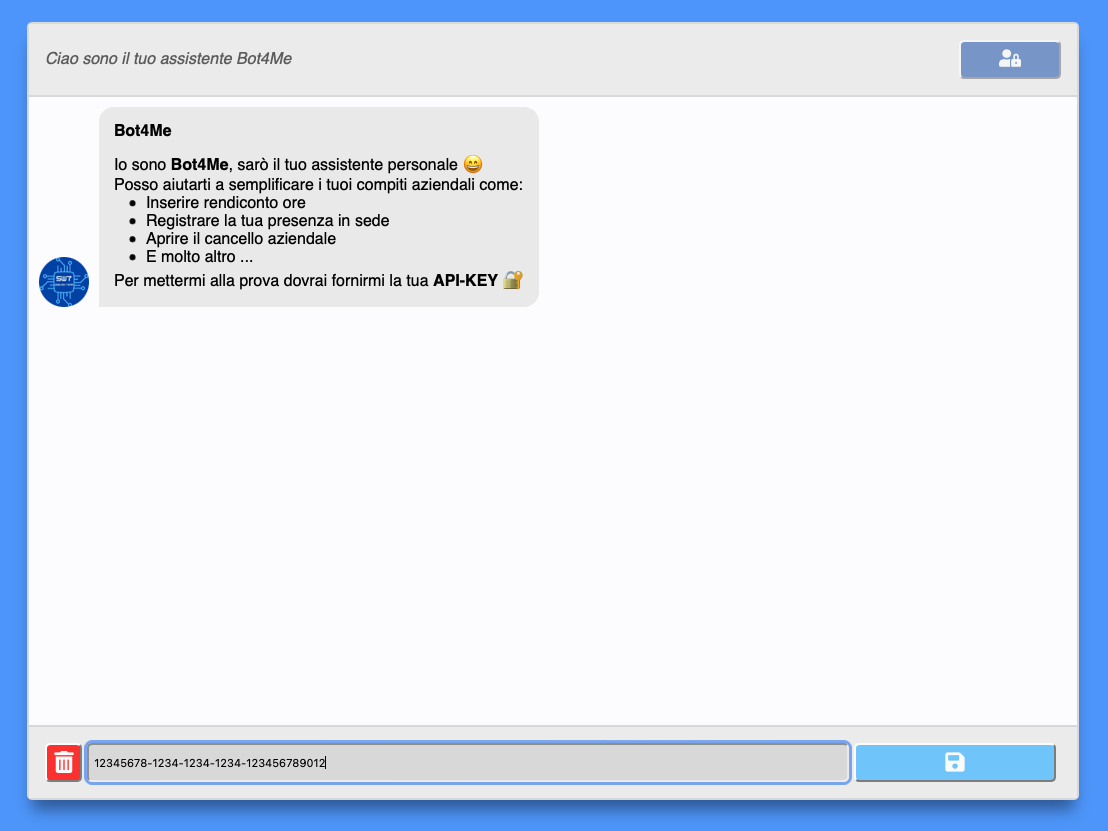
\includegraphics[width=0.9\textwidth, height=0.7\textheight, keepaspectratio]{images/schermata_autenticazione.png}
    \caption{Schermata Autenticazione Bot4me - Inserimento API-KEY}
\end{figure}

\newpage

\subsubsection{Autenticazione - Inserimento \glossario{API-KEY} Non Valida}
\begin{figure}[H]
    \centering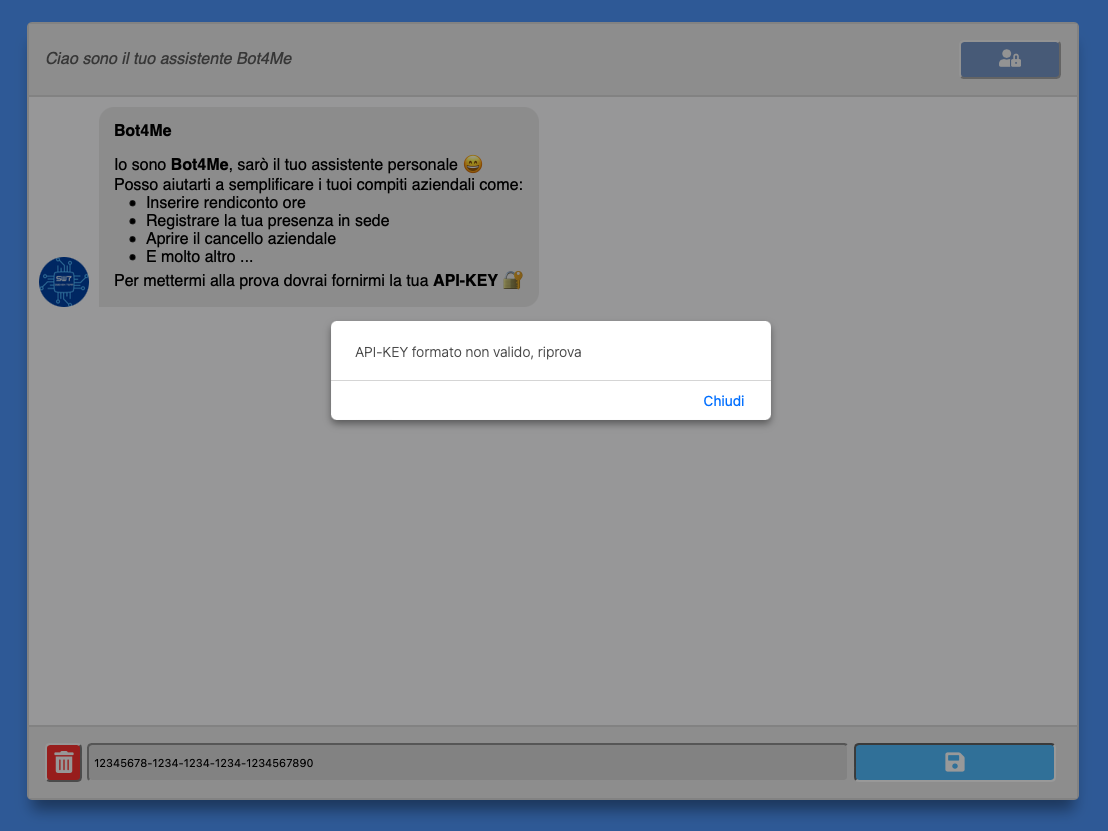
\includegraphics[width=0.9\textwidth, height=0.7\textheight, keepaspectratio]{images/schermata_autenticazione_apikey_non_valida.png}
    \caption{Schermata Autenticazione Bot4me - Inserimento API-KEY Non Valida}
\end{figure}

\subsubsection{Autenticazione Avvenuta con Successo - Inserimento \glossario{API-KEY} Valida e Corretta}
\begin{figure}[H]
    \centering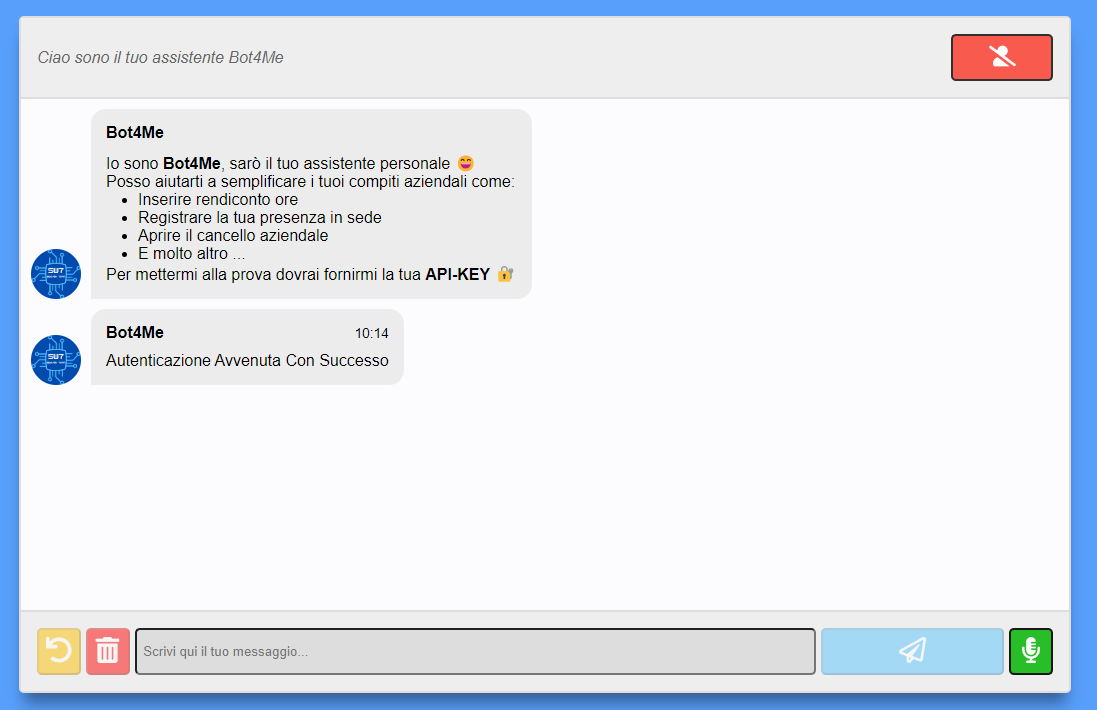
\includegraphics[width=0.9\textwidth, height=0.7\textheight, keepaspectratio]{images/schermata_autenticazione_successo.png}
    \caption{Schermata Autenticazione Avvenuta con Successo Bot4me - Inserimento API-KEY Valida e Corretta}
\end{figure}

\newpage
\section{Descrizione funzionalità}
\subsection{Presenza in Sede}
Dopo essersi autenticati è possibile registrare la propria presenza in sede scrivendo "Presenza" e il chatbot comunica l'avvio dell'operazione richiedendo il nome di una sede. 
Quindi si scrive il nome, se il nome fa parte della lista sedi viene accettato e il chatbot conclude l'operazione di registrazione presenza, altrimenti il bot comunica che la sede non è stata accettata e si invita a reinserire il nome. 
\subsubsection{Schermata Registrazione Presenza - Avvenuta con Successo}
\begin{figure}[H]
    \centering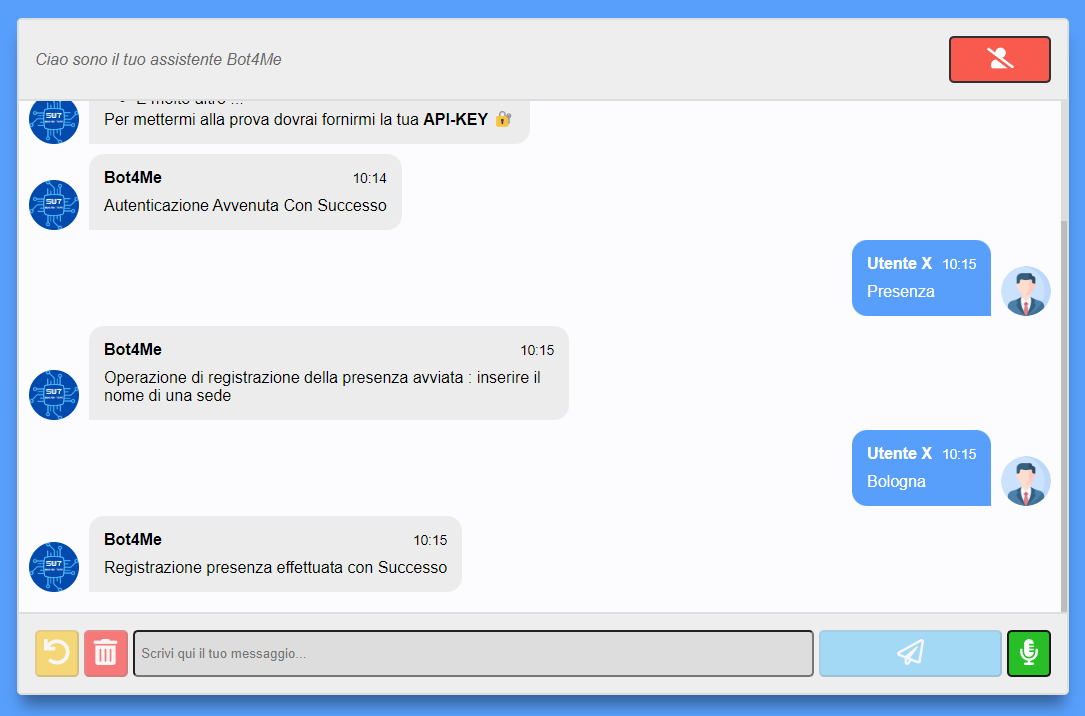
\includegraphics[width=0.9\textwidth, height=0.7\textheight, keepaspectratio]{images/schermata_presenza_successo.png}
    \caption{Schermata Dialogo Registrazione Presenza - Avvenuta con Successo}
\end{figure}

\subsubsection{Schermata Registrazione Presenza - Fallita}
\begin{figure}[H]
    \centering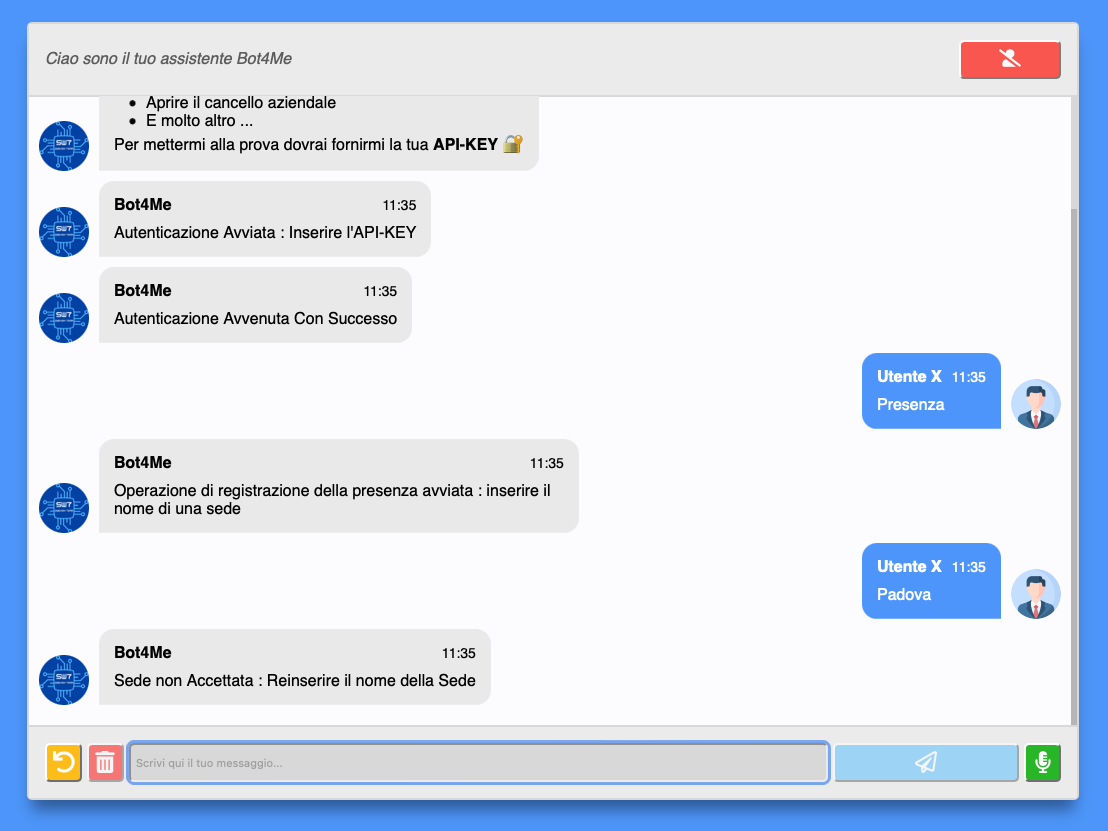
\includegraphics[width=0.9\textwidth, height=0.7\textheight, keepaspectratio]{images/schermata_presenza_fallita.png}
    \caption{Schermata Dialogo Registrazione Presenza - Fallita}
\end{figure}
\newpage
\subsection{Creazione di un nuovo progetto}
Dopo essersi autenticati è possibile creare un nuovo progetto, la richiesta di questa operazione si avvia tramite la parola chiave "crea progetto", quindi il chatbot avvia la creazione e tramite vari messaggi di botta e risposta chiede tutte le informazioni necessarie:
\begin{itemize}
    \item inserire il codice del progetto (se il codice è libero fa proseguire altrimenti chiede un altro codice);
    \item inserire una descrizione;
    \item inserire cliente;
    \item inserire manager;
    \item inserire area (nel senso di luogo);
    \item inserire data inizio;
    \item inserire data fine;
\end{itemize}
Se si inserisce un formato o una parola non valida chiede di reinserire, infine riepiloga tutti i dati ricevuti e chiede conferma se procedere o se si vuole modificare qualche dato o se si vuole annullare la creazione del progetto.

\subsubsection{Schermate Creazione Progetto}
\begin{figure}[H]
    \centering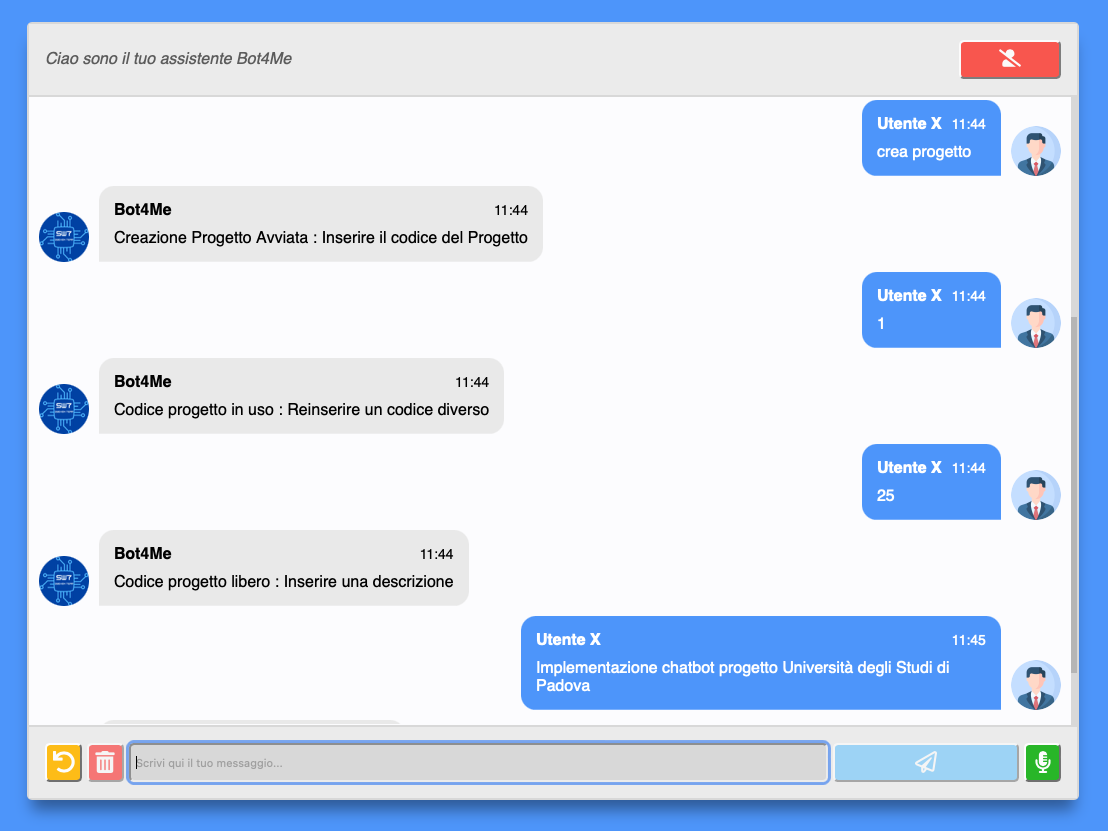
\includegraphics[width=0.8\textwidth, height=0.7\textheight, keepaspectratio]{images/schermata_creazione_progetto_1.png}
    \caption{Schermata Creazione Progetto - Con Inserimento Codice Pre-Esistente}
\end{figure}

\begin{figure}[H]
    \centering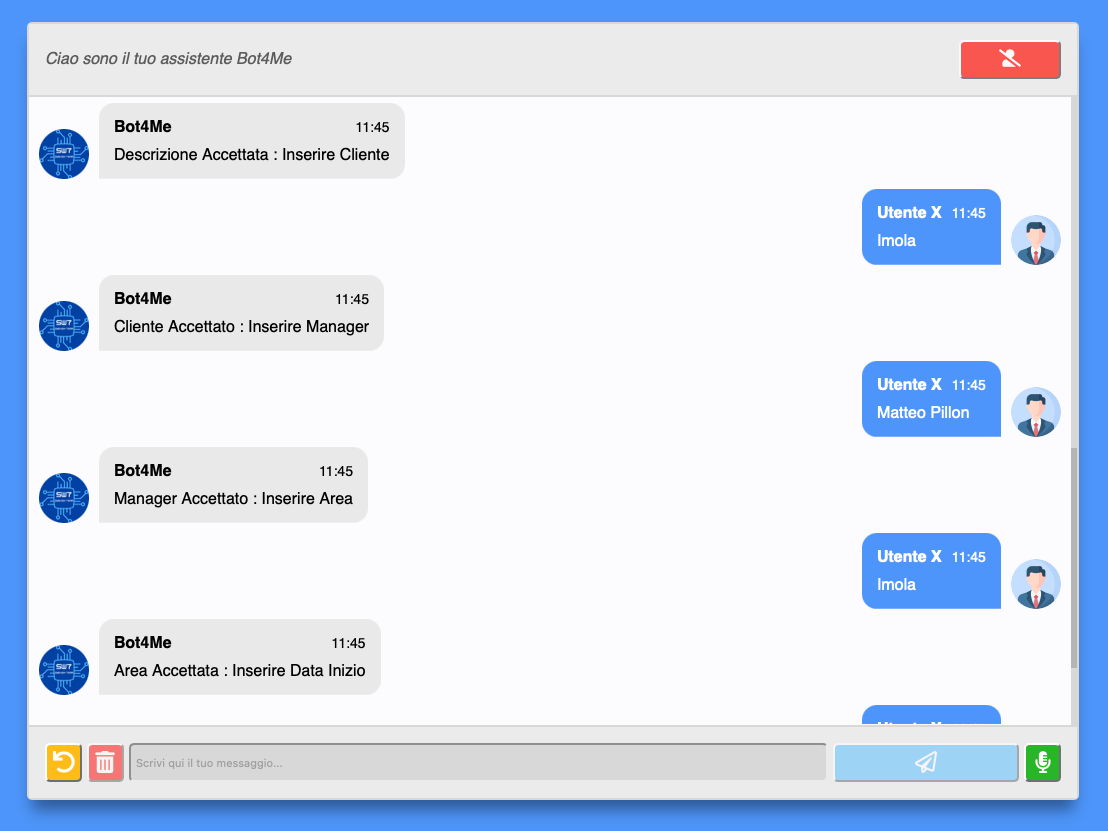
\includegraphics[width=0.8\textwidth, height=0.7\textheight, keepaspectratio]{images/schermata_creazione_progetto_2.png}
    \caption{Schermata Creazione Progetto}
\end{figure}

\begin{figure}[H]
    \centering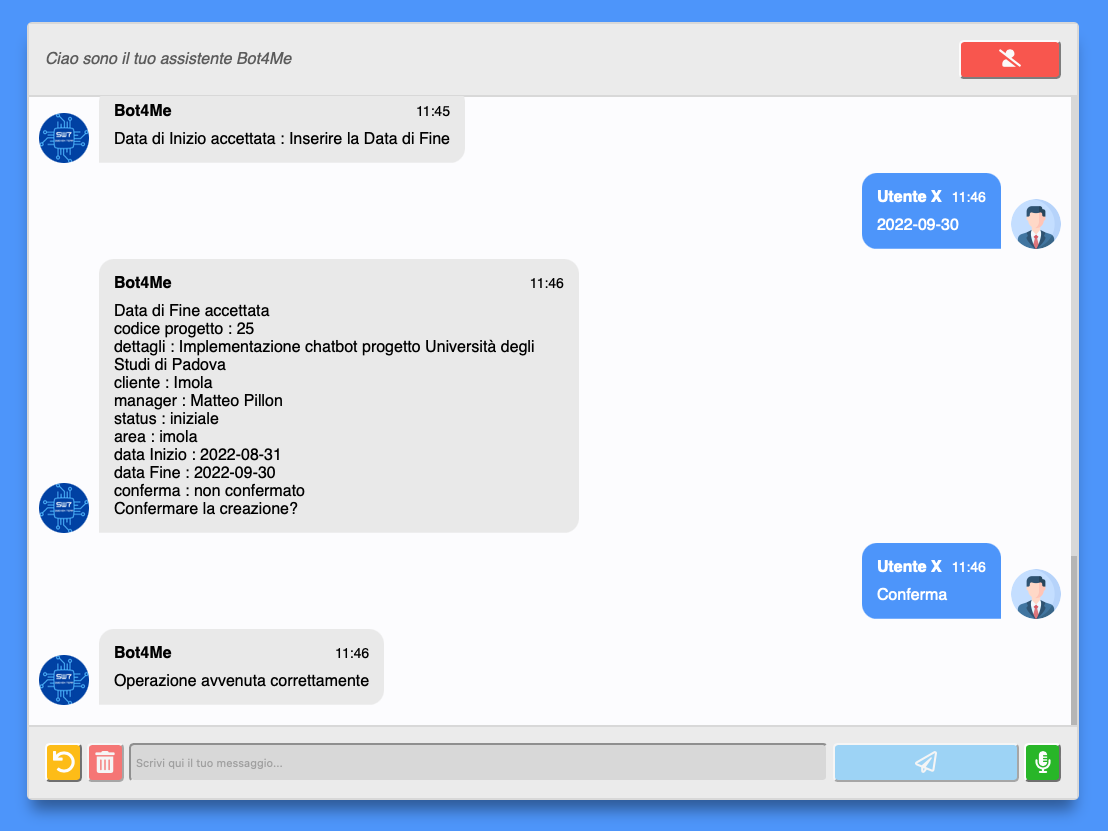
\includegraphics[width=0.8\textwidth, height=0.7\textheight, keepaspectratio]{images/schermata_creazione_progetto_3.png}
    \caption{Schermata Creazione Progetto - Riepilogo e Conferma Operazione}
\end{figure}
\newpage
\subsection{Consuntivazione}
Dopo essersi autenticati è possibile consuntivare le proprie ore di lavoro su un determinato progetto, la richiesta di questa operazione si avvia tramite la parola chiave "consuntiva", quindi il chatbot avvia la consuntivazione e tramite vari messaggi di botta e risposta chiede tutte le informazioni necessarie:
\begin{itemize}
    \item inserire il codice del progetto;
    \item inserire la data di consuntivazione;
    \item inserire le ore fatturabili;
    \item inserire le ore di viaggio;
    \item inserire le ore di viaggio fatturabili;
    \item inserire la sede;
\end{itemize}
Se si inserisce un formato o una parola non valida chiede di reinserire, infine riepiloga tutte le informazioni ricevute e chiede conferma se procedere o se si vuole modificare qualche dato o se si vuole annullare la consuntivazione. 
\subsubsection{Schermate Dialogo Consuntivazione Attività}
\begin{figure}[H]
    \centering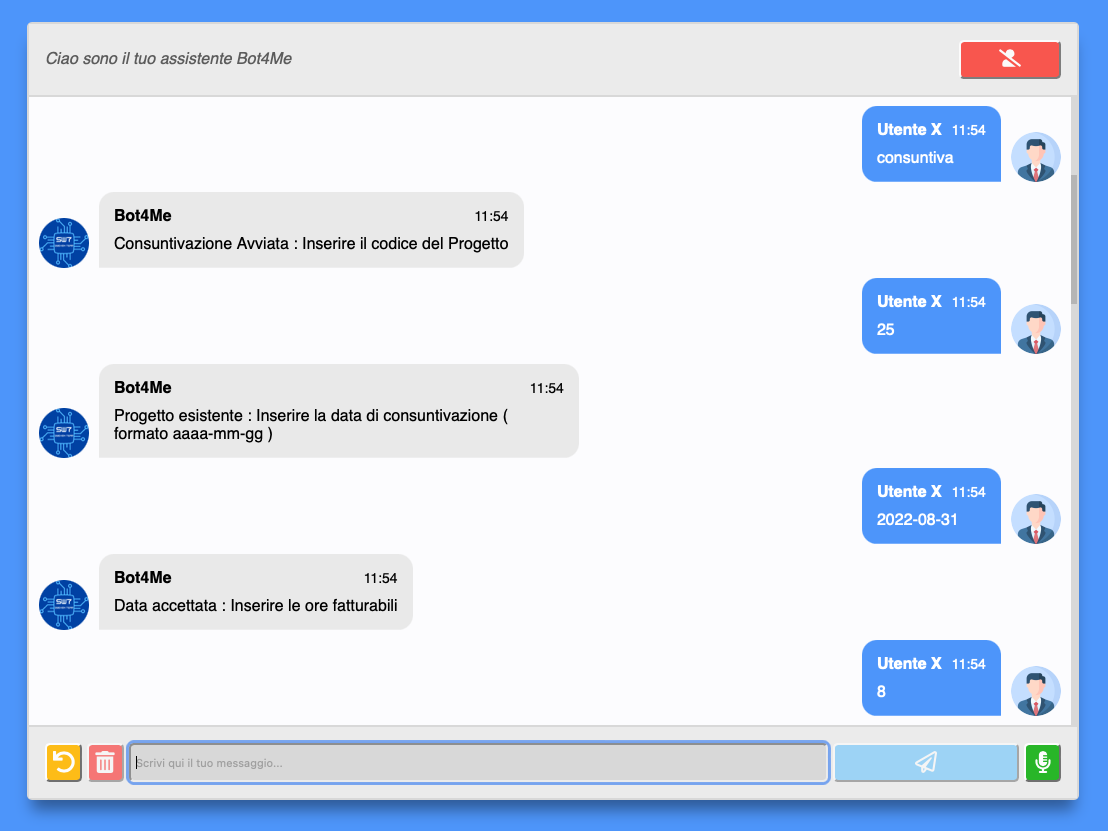
\includegraphics[width=0.9\textwidth, height=0.7\textheight, keepaspectratio]{images/schermata_consultivazione_1.png}
    \caption{Schermata Dialogo Consuntivazione Attività}
\end{figure}

\begin{figure}[H]
    \centering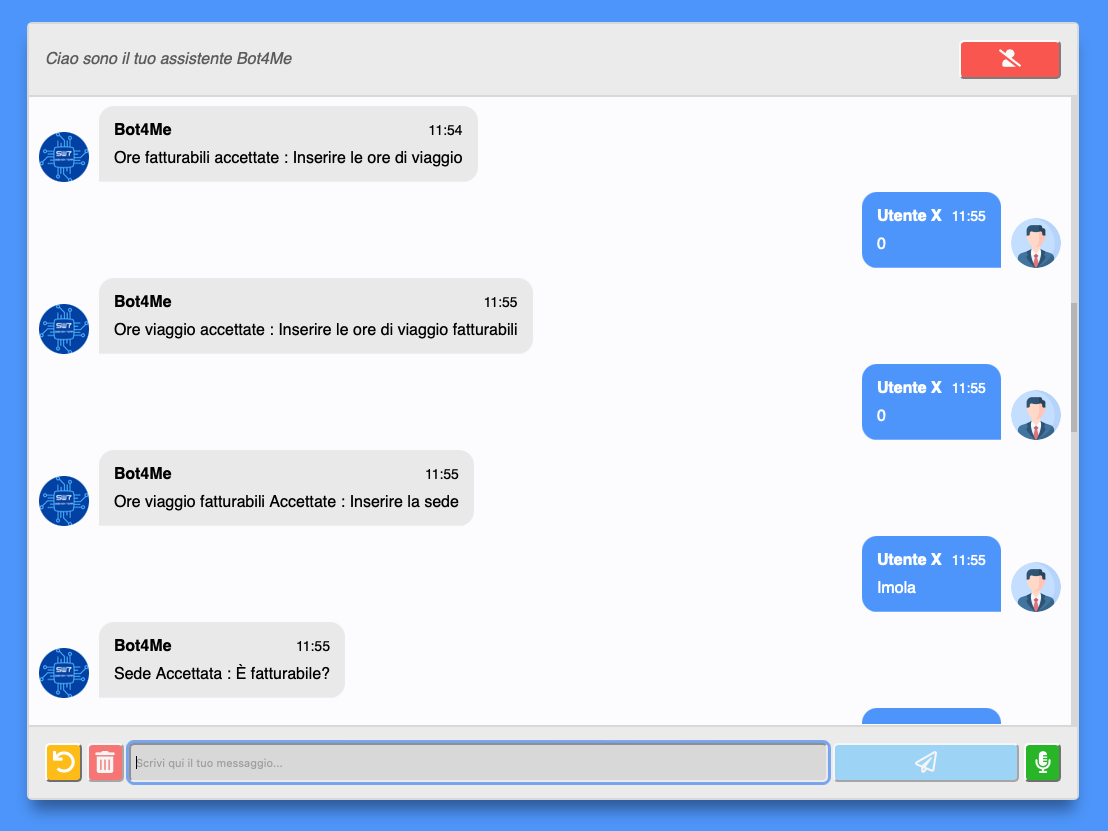
\includegraphics[width=0.9\textwidth, height=0.7\textheight, keepaspectratio]{images/schermata_consultivazione_2.png}
    \caption{Schermata Dialogo Consuntivazione Attività}
\end{figure}

\begin{figure}[H]
    \centering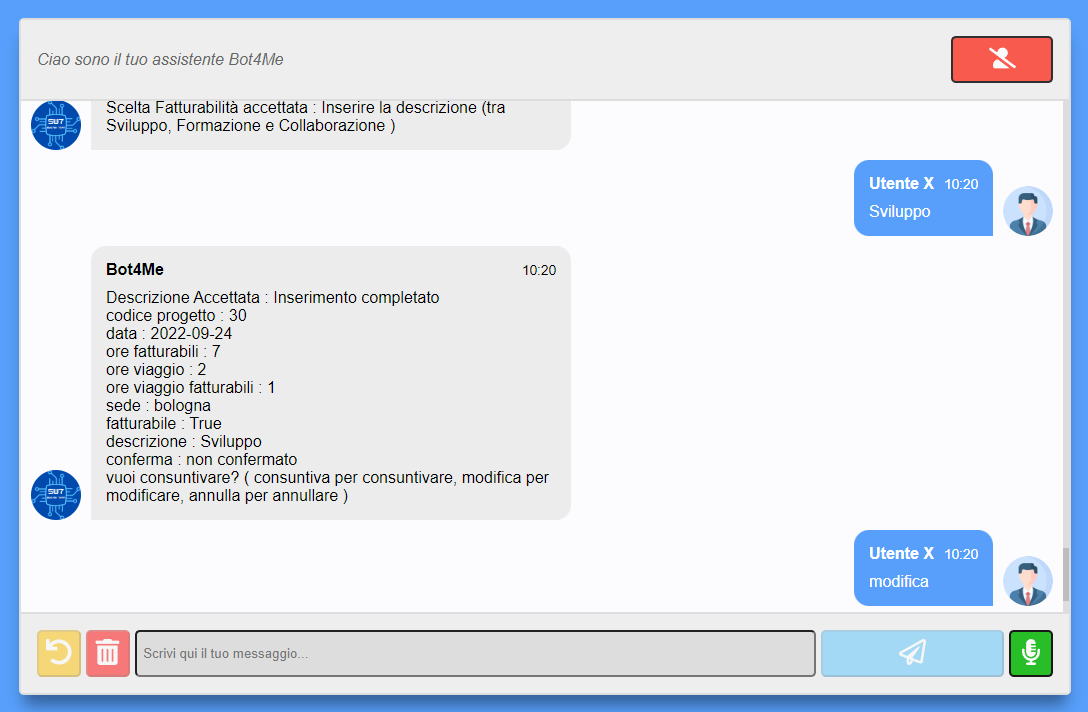
\includegraphics[width=0.8\textwidth, height=0.7\textheight, keepaspectratio]{images/schermata_consultivazione_3.png}
    \caption{Schermata Dialogo Consuntivazione Attività - Modifica Valore}
\end{figure}

\begin{figure}[H]
    \centering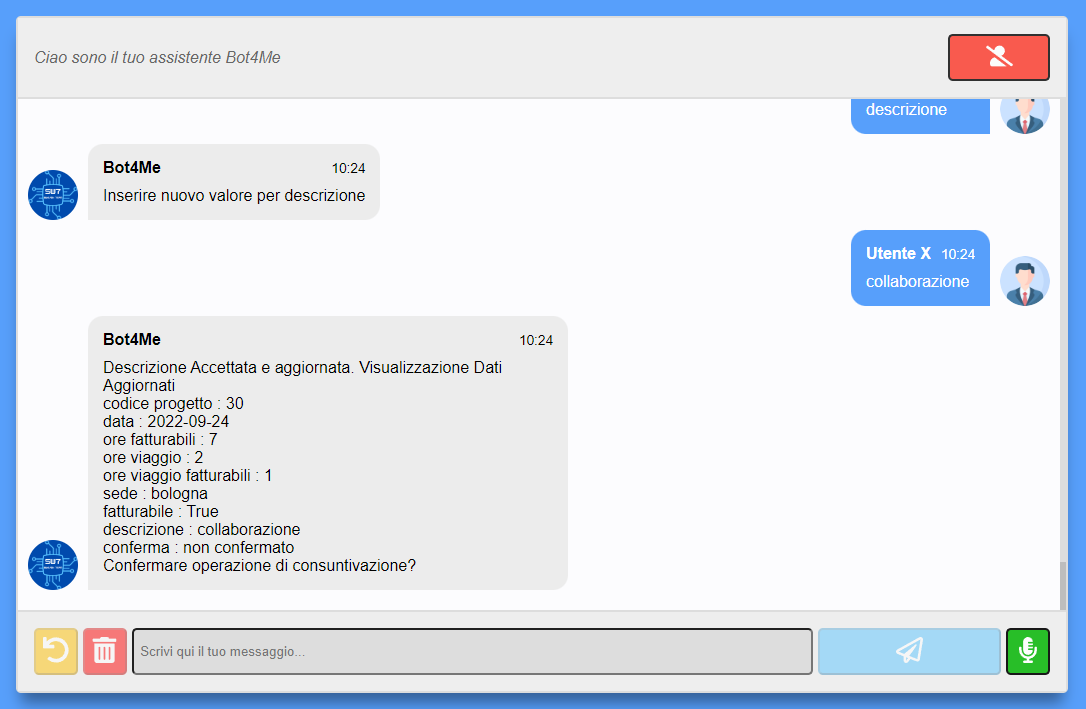
\includegraphics[width=0.8\textwidth, height=0.7\textheight, keepaspectratio]{images/schermata_consultivazione_4.png}
    \caption{Schermata Dialogo Consuntivazione Attività - Nuovo Valore Descrizione Attività}
\end{figure}

\begin{figure}[H]
    \centering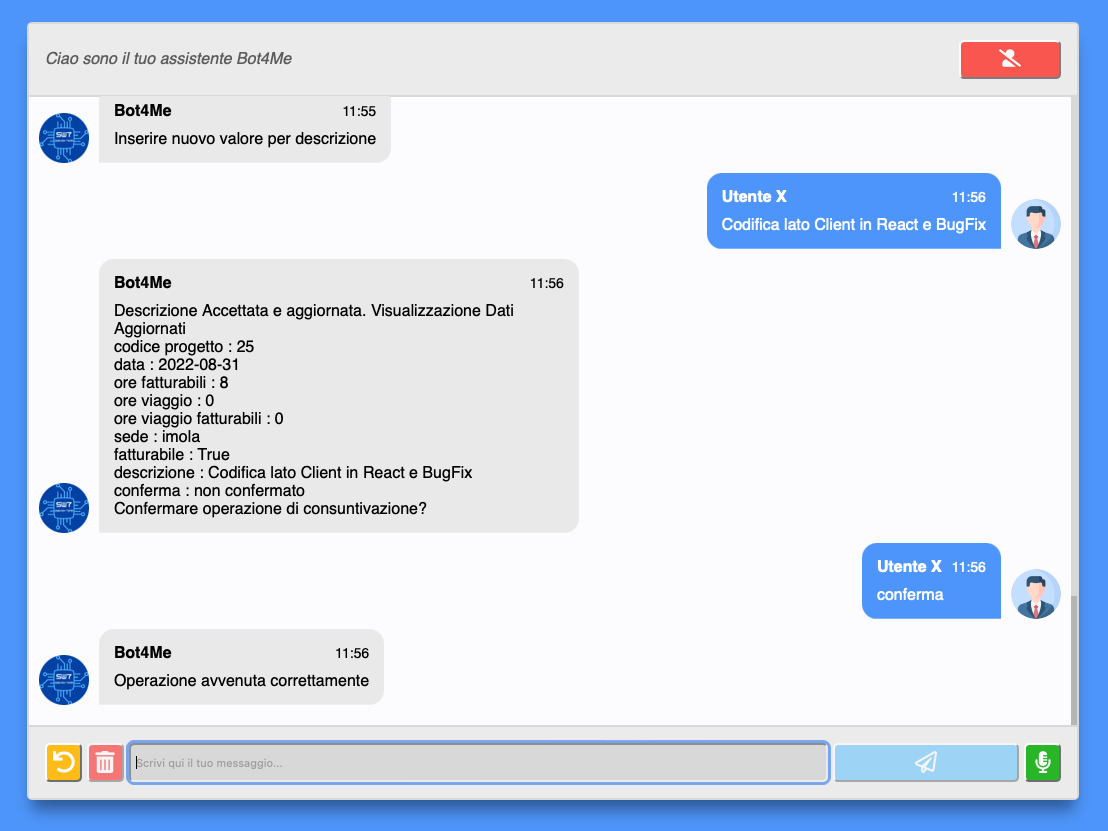
\includegraphics[width=0.9\textwidth, height=0.7\textheight, keepaspectratio]{images/schermata_consultivazione_5.png}
    \caption{Schermata Dialogo Consuntivazione Attività - Conferma Operazione}
\end{figure}
\newpage
\subsubsection{Vedere le consuntivazioni per un progetto}
Dopo essersi autenticati è possibile richiedere la visione delle consuntivazioni effettuate su un determinato progetto scrivendo "ottieni consuntivazione", poi verrà richiesto di inserire il codice del progetto e il chatbot risponderà con un lungo messaggio contenente tutte le consuntivazioni effettuate, al momento della stesura di questo documento non è possibile filtrare le consultivazioni per un dato per periodo. 
\begin{figure}[H]
    \centering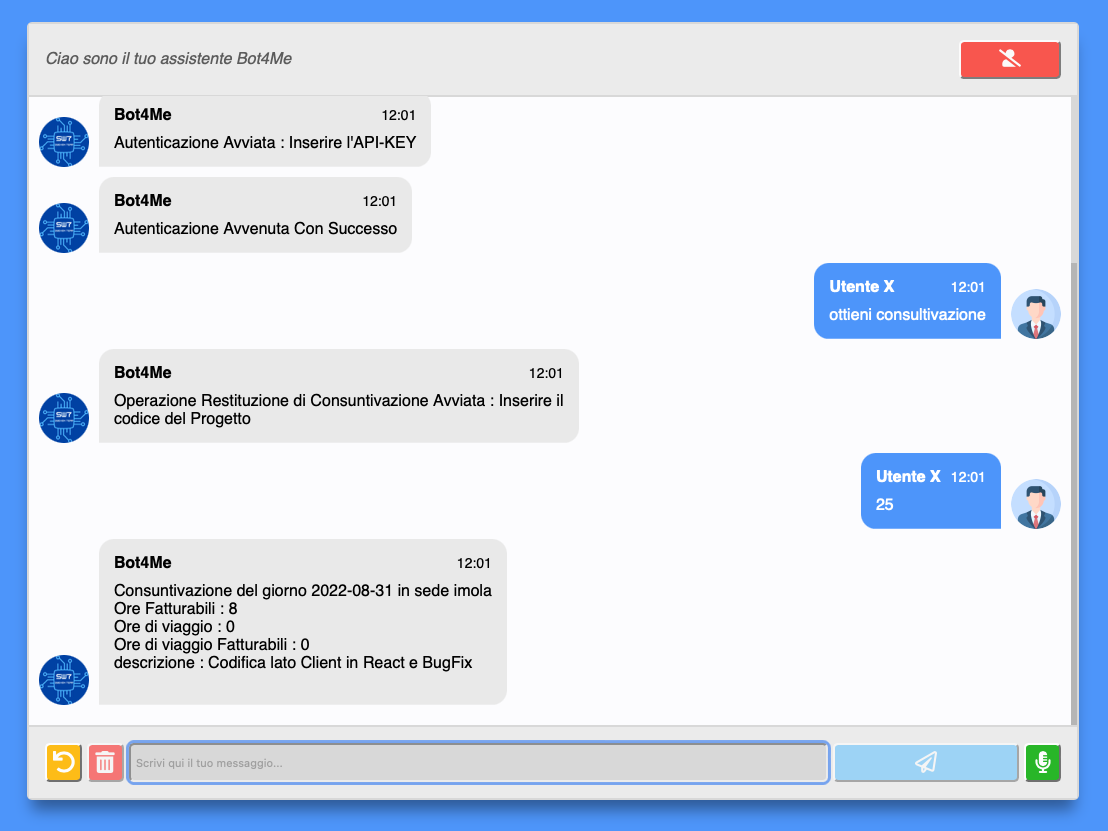
\includegraphics[width=0.9\textwidth, height=0.7\textheight, keepaspectratio]{images/schermata_ottieni_consultivazione.png}
    \caption{Schermata Dialogo Ottenimento Consuntivazioni Registrate per Progetto}
\end{figure}
\newpage
\subsection{Apertura Cancello}
Dopo essersi autenticati è possibile richiedere l'apertura del cancello di una determinata sede scrivendo "apertura cancello" e il chatbot chiederà in quale sede, dopo aver inserito la sede il chatbot chiede se si vuole confermare, modificare o annullare e in caso di conferma procede con l'apertura.

\begin{figure}[H]
    \centering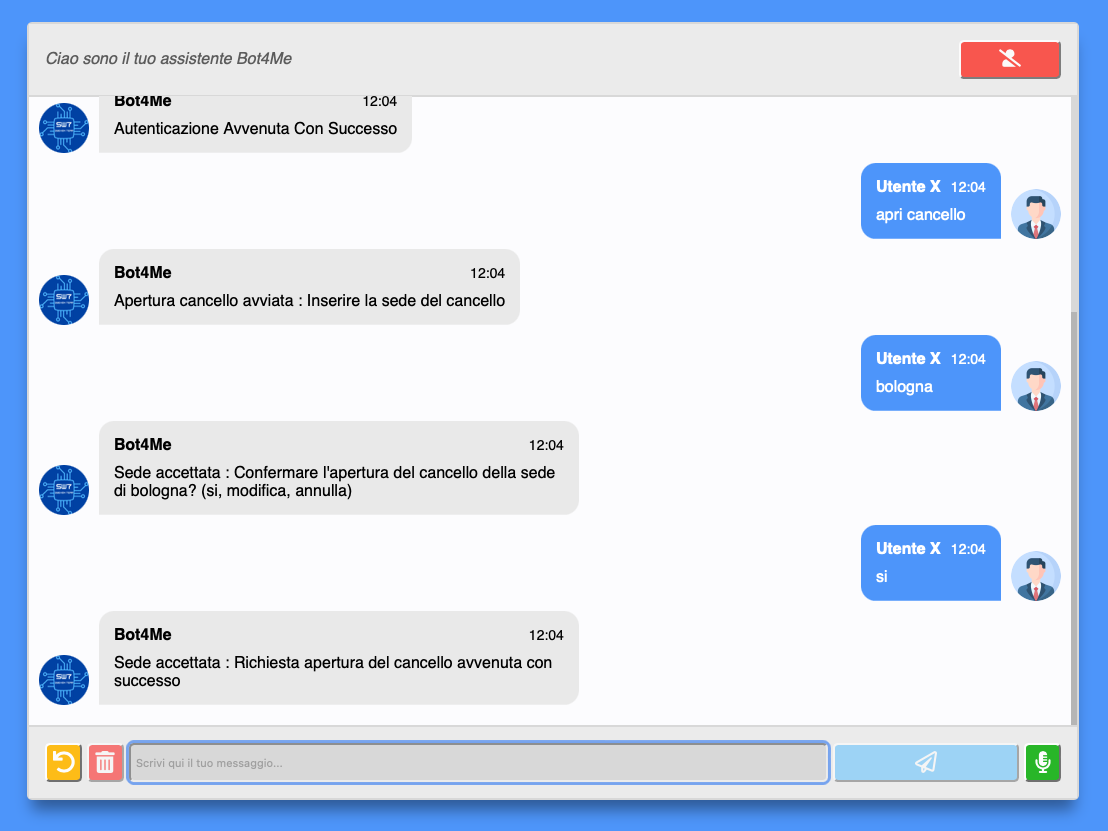
\includegraphics[width=0.9\textwidth, height=0.7\textheight, keepaspectratio]{images/schermata_apertura_cancello.png}
    \caption{Schermata Dialogo Apertura Cancello}
\end{figure}
\newpage
\section{Supporto}
Nel caso venissero riscontrati bug o malfunzionamenti, si prega di inviare una mail all’indirizzo 
\href{mailto:swe7.team@gmail.com}{\color{blue}swe7.team@gmail.com} \newline 
La mail deve essere preferibilmente nel seguente formato:
\begin{itemize}
    \item \textbf{Oggetto:} Nome dell’evento da segnalare;
    \item \textbf{Corpo:} 
        \begin{itemize}
            \item data in cui è stato riscontrato il problema;
            \item breve descrizione del problema;
            \item sistema operativo e browser in cui è avvenuto il problema;
        \end{itemize}
    \item \textbf{Allegati:} è possibile allegare immagini o contenuto testuale che possa facilitare la risoluzione del problema
\end{itemize}
In alternativa, è possibile contattarci tramite l’organizzazione di \glossario{Github} al seguente link:
\href{https://github.com/SwevenTeam}{\color{blue} https://github.com/SwevenTeam} 

\end{document}
